%% Author: Julie Hoffer
%% Subject: Metastudies

Here is a diagram from the {\em Essential Epidemiology} textbook:

\centerline{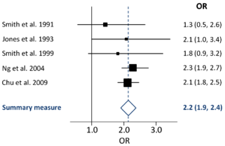
\includegraphics[width=3in]{metastudy.png}}

In referring to the individual studies, you can use names like ``Smith 1991'' or ``Jones 1993''.

\begin{enumerate}

\item Which study/studies have the largest weight in this meta analysis?

\begin{AnswerText} 
Ng 2004 and Chu 2009
\end{AnswerText}

\item Which studies individually do {\bf not} show statistical significance?

\begin{AnswerText} 
Smith, 1991  Smith, 1999 and Jones 1993
\end{AnswerText}

\item What is the odds ratio for the meta analysis of the studies?

\begin{AnswerText} 
2.0
\end{AnswerText}

\item What is the purpose of a meta analysis?

\begin{AnswerText} 
Integrate findings from a large number of studies with the same study outcome.
\end{AnswerText}

\end{enumerate}
